\documentclass[handout]{beamer}
\usepackage{amsmath}
\usepackage{graphicx}
\usepackage{hyperref}
\usepackage{listings}
\usepackage{ragged2e}
\usepackage[utf8]{inputenc}
\usepackage{xcolor}

\justifying % Justify text in frames by default

%------------------------------------------------------------------------------
%   THEME AND COLOR DEFINITIONS (LAPAN BRANDING)
%------------------------------------------------------------------------------
\usetheme{Boadilla}

% --- Custom LAPAN Colors ---
%\definecolor{LAPANorange}{RGB}{243, 112, 33}
%\definecolor{LAPANgray}{RGB}{105, 105, 105}
\definecolor{LAPANorange}{HTML}{FF6600} % A vibrant orange
\definecolor{LAPANgray}{RGB}{105, 105, 105}
\definecolor{lapanblue}{HTML}{F0F0F0}   % A light gray for backgrounds
\definecolor{lapanorange}{HTML}{FF6600} % A vibrant orange
\definecolor{lapangray}{HTML}{F0F0F0}   % A light gray for backgrounds

% --- Applying Custom Colors to Beamer Elements ---
\setbeamercolor{normal text}{fg=black, bg=white}
\setbeamercolor{structure}{fg=LAPANorange}
\setbeamercolor{frametitle}{bg=LAPANgray, fg=white}
\setbeamercolor{title}{bg=LAPANgray, fg=white}
\setbeamercolor{palette primary}{bg=LAPANorange, fg=white}
\setbeamercolor{palette secondary}{bg=LAPANgray, fg=white}
\setbeamercolor{palette tertiary}{bg=LAPANgray, fg=white}
\setbeamercolor{palette quaternary}{bg=LAPANorange, fg=white}
\setbeamercolor{section in sidebar}{fg=white, bg=LAPANgray}
\setbeamercolor{subsection in sidebar}{fg=white, bg=LAPANgray!75}
\setbeamercolor{block title}{bg=LAPANorange, fg=white}
\setbeamercolor{block body}{bg=LAPANgray!20, fg=black}
\setbeamercolor{alerted text}{fg=LAPANorange}


% Python code listing style
\lstdefinestyle{pythonstyle}{
	language=Python,
	backgroundcolor=\color{lapangray},
	commentstyle=\color{gray},
	keywordstyle=\color{lapanblue},
	stringstyle=\color{purple},
	basicstyle=\ttfamily\footnotesize,
	breakatwhitespace=false,
	breaklines=true,
	captionpos=b,
	keepspaces=true,
	numbers=left,
	numbersep=5pt,
	showspaces=false,
	showstringspaces=false,
	showtabs=false,
	tabsize=2
}
\lstset{style=pythonstyle}




%------------------------------------------------------------------------------
%   PRESENTATION METADATA
%------------------------------------------------------------------------------
\title[Computational Neuro-Vision]{Computational Methods for Neurosciences of Vision: From Neurons to Actionable Insights}
\author{Hugo de Paula}
\institute[LAPAN]{Laboratório de Pesquisa Aplicada a Neurovisão (LAPAN) \\ Universidade Federal de Minas Gerais (UFMG) \\ Hospital de Olhos de Minas Gerais}
\date{\today}
\titlegraphic{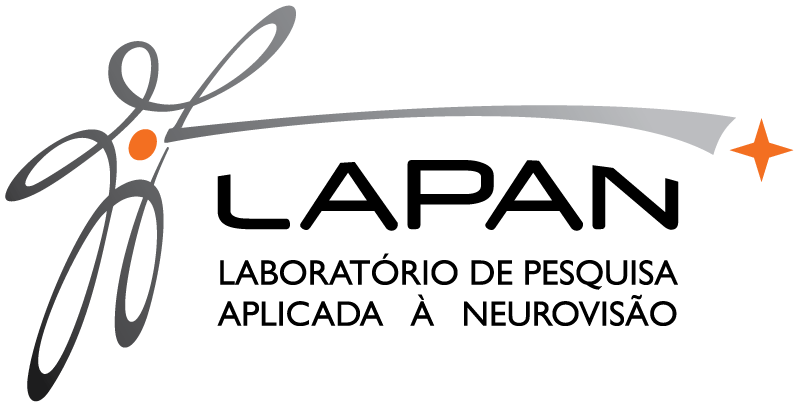
\includegraphics[height=2cm]{lapan.png}}

%------------------------------------------------------------------------------
%   BEGIN DOCUMENT
%------------------------------------------------------------------------------
\begin{document}
	
% --- Title Page ---
\begin{frame}
	\titlepage
\end{frame}

% --- Table of Contents ---
\begin{frame}
	\frametitle{Outline}
	\tableofcontents
\end{frame}
	
	
	
%------------------------------------------------------------------------------
\section{Introduction}
%------------------------------------------------------------------------------

\begin{frame}
	\frametitle{LAPAN's core objectives}
	\begin{columns}
		\begin{column}{0.7\textwidth}
			\begin{itemize}
				\item<1-> \textbf{Innovation:} Develop new technologies for the diagnosis and treatment of vision related disorders.
				\item<2-> \textbf{Research:} Connect basic neuroscientific research with clinical practice.
				\item<3-> \textbf{Health:} Provide tools for early identification and intervention in clinical neuro-ophthalmology.
			\end{itemize}
		\end{column}
		\begin{column}{0.3\textwidth}
			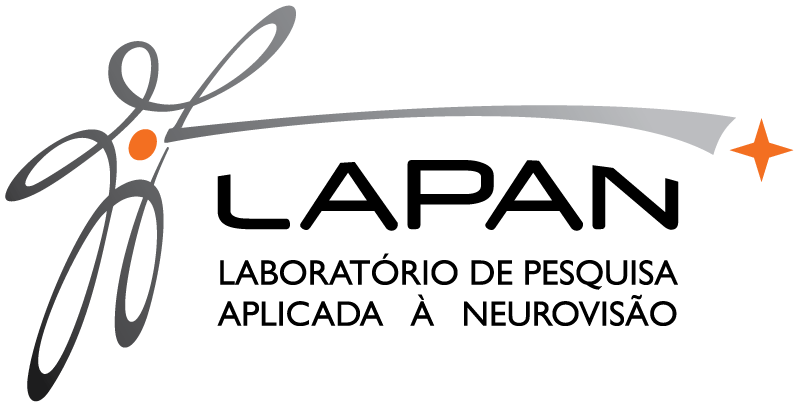
\includegraphics[width=\textwidth]{lapan.png}
		\end{column}
	\end{columns}
\end{frame}


% ===================================================================
\section{The Rational Agent Framework}
% ===================================================================

\begin{frame}
	\frametitle{The Paradigm of Rational Agents}
	In their book, "Artificial Intelligence: A Modern Approach," Stuart Russell and Peter Norvig introduce the concept of a \textbf{rational agent}.
	\begin{itemize}
		\item \textbf{Agent}: Anything that can be viewed as perceiving its environment through \textit{sensors} and acting upon that environment through \textit{actuators}.
		\item \textbf{Rational Agent}: An agent that acts to achieve the \alert{best expected outcome}.
	\end{itemize}
	\vspace{1cm}
	\begin{alertblock}{Application in Neuroscience}
		This framework provides a powerful structure for understanding biological systems, including the visual system, as agents striving to make optimal decisions based on sensory input.
	\end{alertblock}
\end{frame}


\begin{frame}
	\frametitle[PEAS Framework]{PEAS Framework:  \textbf{P}erformance, \textbf{E}nvironment, \textbf{A}ctuators, \textbf{S}ensors}
	
	\begin{figure}
		\centering
		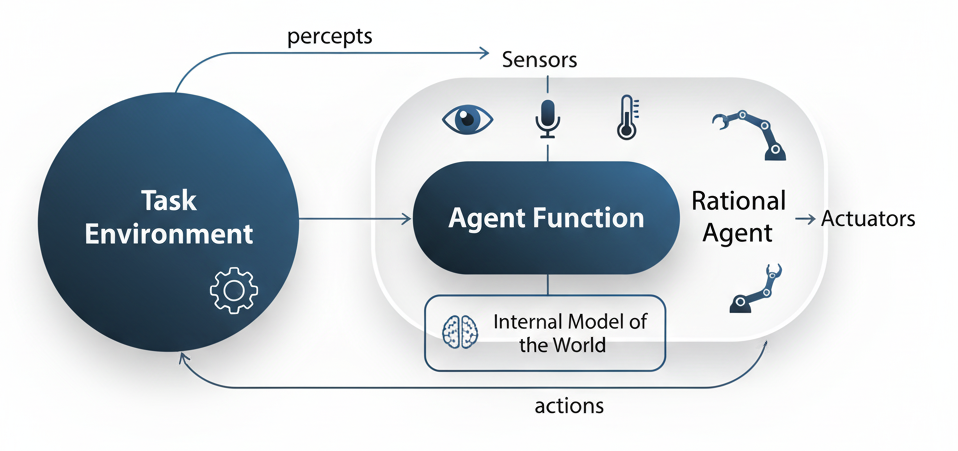
\includegraphics[width=.75\textwidth]{figures/rational_agents.png}
	\end{figure}
	\begin{itemize}
		\item \textbf{Sensors}: How the agent perceives the environment (e.g., retinal photoreceptors, EEG electrodes, fMRI scanner).

		\item \textbf{Actuators}: How the agent acts on the environment (e.g., eye muscle contractions, verbal response, clinical diagnosis).
	\end{itemize}
\end{frame}



\begin{frame}
	\frametitle[PEAS Framework]{PEAS Framework:  \textbf{P}erformance, \textbf{E}nvironment, \textbf{A}ctuators, \textbf{S}ensors}
	
	\begin{figure}
		\centering
		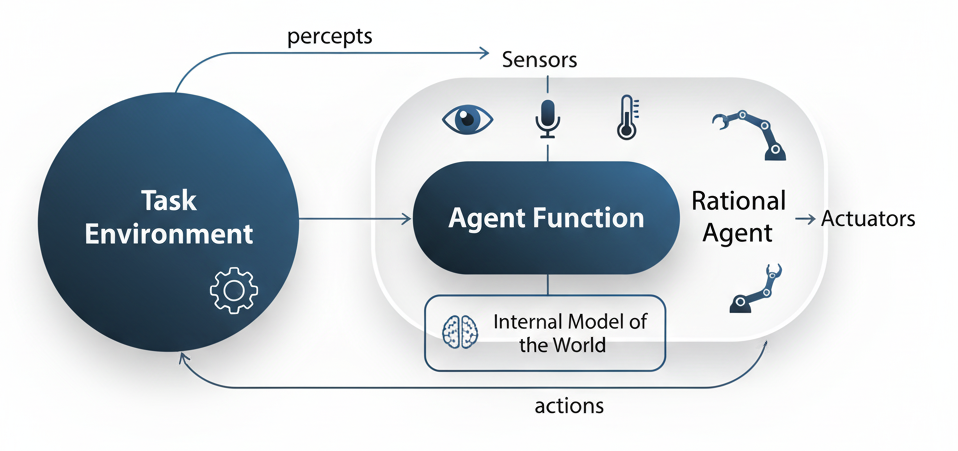
\includegraphics[width=.75\textwidth]{figures/rational_agents.png}
	\end{figure}

	\begin{itemize}
		\item \textbf{Environment}: The context in which the agent operates (e.g., a cluttered visual scene, clinical setting).

		\item \textbf{Performance Measure}: What defines success? (e.g., accuracy in identifying an object, speed of reaction).
	\end{itemize}
\end{frame}

% ===================================================================
\section{Agent Function and Learning}
% ===================================================================

\begin{frame}
	\frametitle{Building the Agent Function}
	The core of a rational agent is the \textbf{agent function}, which maps percept sequences to actions.
	\begin{center}
		$f: P^* \rightarrow A$
	\end{center}
	Where $P^*$ is the set of all possible percept sequences and $A$ is the set of all possible actions.
	
	\vspace{1cm}
	
	\begin{alertblock}{Our Goal}
		To use computational methods to model or approximate this function for specific tasks in visual neuroscience. We want to understand how the brain turns sensory data into meaningful action.
	\end{alertblock}
\end{frame}

\begin{frame}
	\frametitle[The Agent Function]{The Agent Function: Learning from Data}
	\begin{itemize}
		\item \textbf{Agent Function:} Maps input data (percepts) to optimal actions.
		\item \textit{Simple:} IF-THEN rules.
		\item \textit{Complex:} Data-driven machine learning models.
	\end{itemize}
	\pause
	\begin{alertblock}{Model Fitting \& Common Tasks}
		\begin{itemize}
			\item \textbf{Classification:} Assign category (e.g., healthy/diseased).
			\item \textbf{Regression:} Predict value (e.g., disease severity score).
			\item \textbf{Recommendation:} Suggest treatments or interventions.
		\end{itemize}
	\end{alertblock}
\end{frame}

\begin{frame}
	\frametitle{Deep Learning: Artificial Neural Networks as Models of Vision}
	\begin{itemize}
		\item \textbf{Convolutional Neural Networks (CNNs)} deep learning models inspired by the architecture of the mammalian visual cortex.
		\item Layers of artificial neurons learn to detect features in a hierarchical manner, from simple edges to complex objects.
		\item Remarkably, the internal representations learned by CNNs trained on object recognition tasks show a striking similarity to the representations found in the primate ventral visual stream.
	\end{itemize}
	\begin{figure}
		\centering
		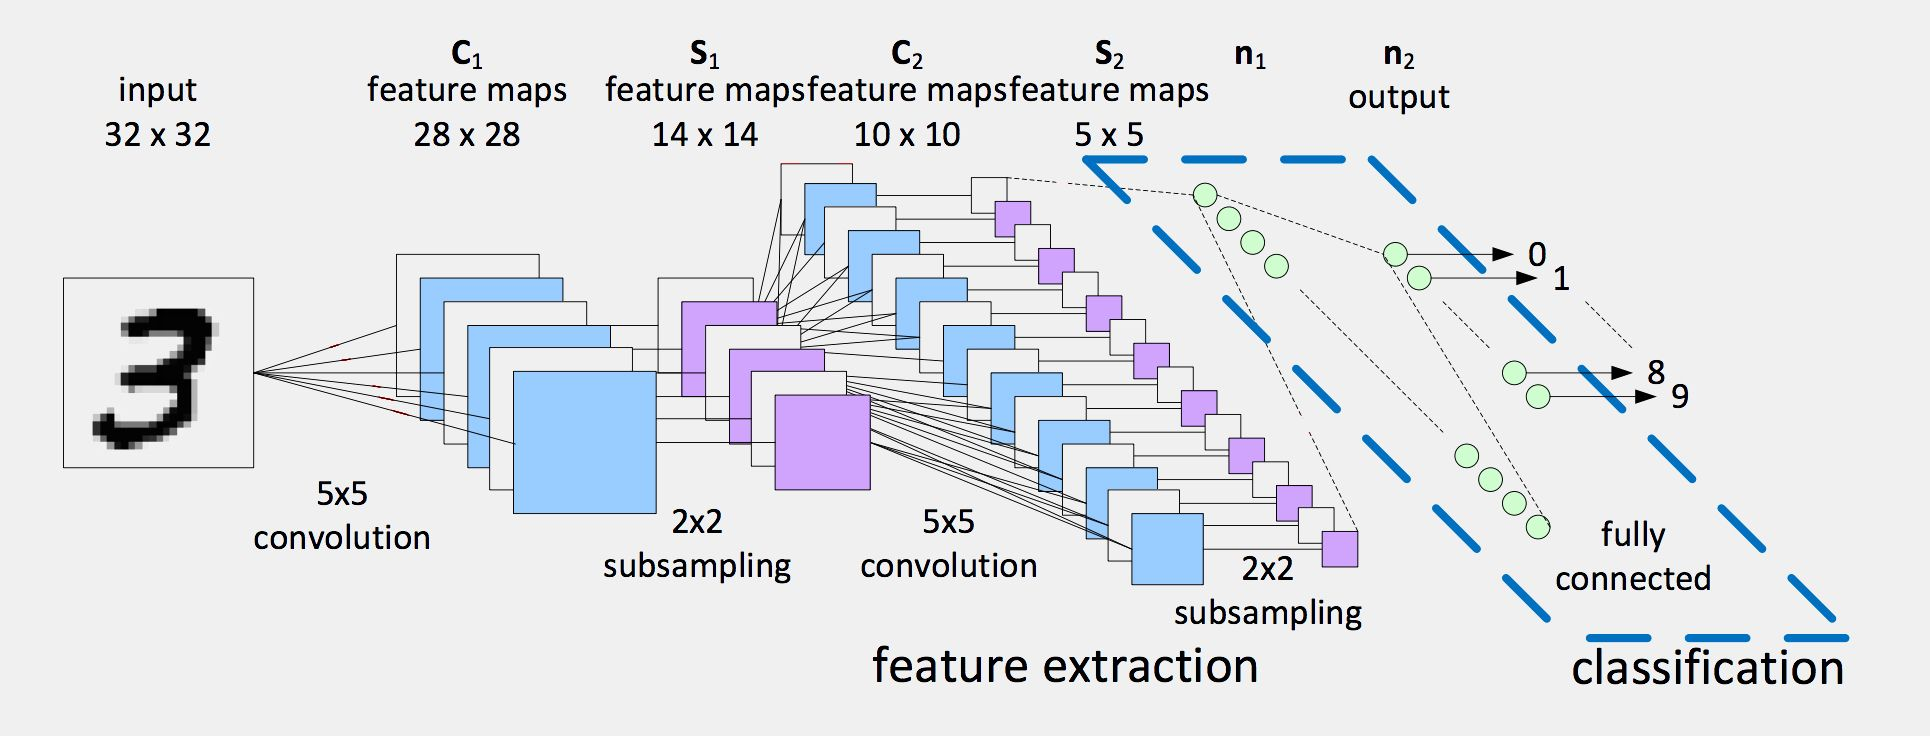
\includegraphics[width=.7\textwidth]{figures/cnn_architecture.jpg}
		\caption{\tiny 
			Peemen, M. C. J., Mesman, B., \& Corporaal, H. (2011). Speed sign detection and recognition by convolutional neural networks. In Proceedings of the 8th International Automotive Congress (IAC 2011).}
	\end{figure}
\end{frame}


\begin{frame}
	\frametitle{Sensors: Features and Descriptors}
	Raw sensor data (like an EEG signal) is often too complex. We extract \textbf{features} to represent the data in a more informative way.
	\begin{columns}
		\begin{column}{0.5\textwidth}
		\textbf{Temporal Domain}
		\begin{itemize}
			\item Amplitude, Latency, Zero-crossings
		\end{itemize}
		\textbf{Frequency Domain} (via FFT)
		\begin{itemize}
			\item Power in specific bands ($\delta, \theta, \alpha, \beta, \gamma$)
			\item Peak frequency
		\end{itemize}
		\textbf{Time-Frequency Domain} (via Wavelets, Spectrograms)
		\end{column}
		\begin{column}{0.5\textwidth}
			\begin{figure}
				\centering
				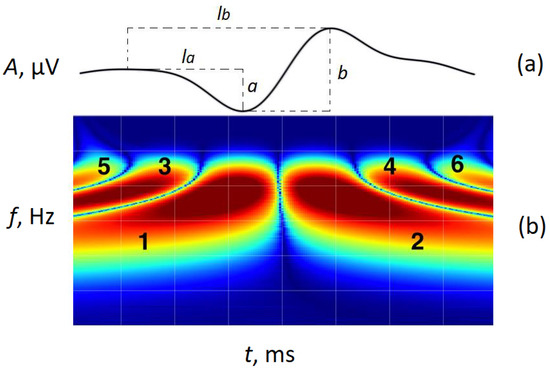
\includegraphics[width=\textwidth]{figures/wavelet.jpg}
				\caption{\tiny Zhdanov, A.; Dolganov, A.; Zanca, D.; Borisov, V.; Ronkin, M. Advanced Analysis of Electroretinograms Based on Wavelet Scalogram Processing. Appl. Sci. 2022, 12, 12365. https://doi.org/10.3390/app122312365 }
			\end{figure}
		\end{column}
	\end{columns}
\end{frame}


\begin{frame}
	\frametitle{Key Oculomotor Parameters (Eye Movement)}
	Several key parameters that reflect the integrity of the underlying neural circuits:
	\begin{itemize}
		\item \textbf{Saccadic Latency:} The time delay between the appearance of a target and the initiation of the eye movement ($ms$).
		\item \textbf{Peak Velocity:} The maximum speed of the eye during a saccade ($deg/s$). This is related to the "main sequence" of saccades.
		\item \textbf{Saccadic Accuracy:} The precision of the saccade in landing on the target (gain = actual amplitude / target amplitude).
		\item \textbf{Postural Stability:} The ability to maintain balance, which is tightly integrated with the vestibular and visual systems ($mm^2$ of sway area).
	\end{itemize}
\end{frame}
	
\begin{frame}
	\frametitle{Actuators: Translating Outputs to Insights}
	The output of our computational model must be translated into a meaningful action or insight.
	\begin{itemize}
		\item \textbf{Binary Output} (e.g., 0 or 1):
		\begin{itemize}
			\item \textit{Example}: Healthy vs. Impaired.
			\item \textit{Action}: Recommend further testing for the ``Impaired'' class.
		\end{itemize}
		\item \textbf{Multi-Class Output} (e.g., 1, 2, 3):
		\begin{itemize}
			\item \textit{Example}: Identifying object A, B, or C from fMRI data.
			\item \textit{Action}: Decode the subject's visual experience.
		\end{itemize}
		\item \textbf{Continuous Output} (e.g., 1.23, -4.5):
		\begin{itemize}
			\item \textit{Example}: Predicting the severity score of a condition.
			\item \textit{Action}: Triage patients based on the predicted score.
		\end{itemize}
	\end{itemize}
\end{frame}

\begin{frame}
	\frametitle[Performance Metrics]{Performance Metrics: How Good Is Our Agent?}
	\begin{columns}
		\begin{column}{.6\textwidth}
			\textbf{Classification Metrics}:
			\begin{itemize}
				\item \alert{Accuracy}: Overall correct predictions.
				\item \alert{Precision}: Of the positive predictions, how many were correct?
				\item \alert{Recall}: Of all actual positives, how many did we find?
				\item \alert{F1-Score}: The harmonic mean of Precision and Recall.
			\end{itemize}
		\end{column}		
		\begin{column}{.4\textwidth}
			\textbf{Regression Metrics}:
			\begin{itemize}
				\item \alert{RMSE} (Root Mean Squared Error): Penalizes large errors.
				\item \alert{MAE} (Mean Absolute Error): Average error magnitude.
			\end{itemize}
		\end{column}
	\end{columns}
	\begin{center}
		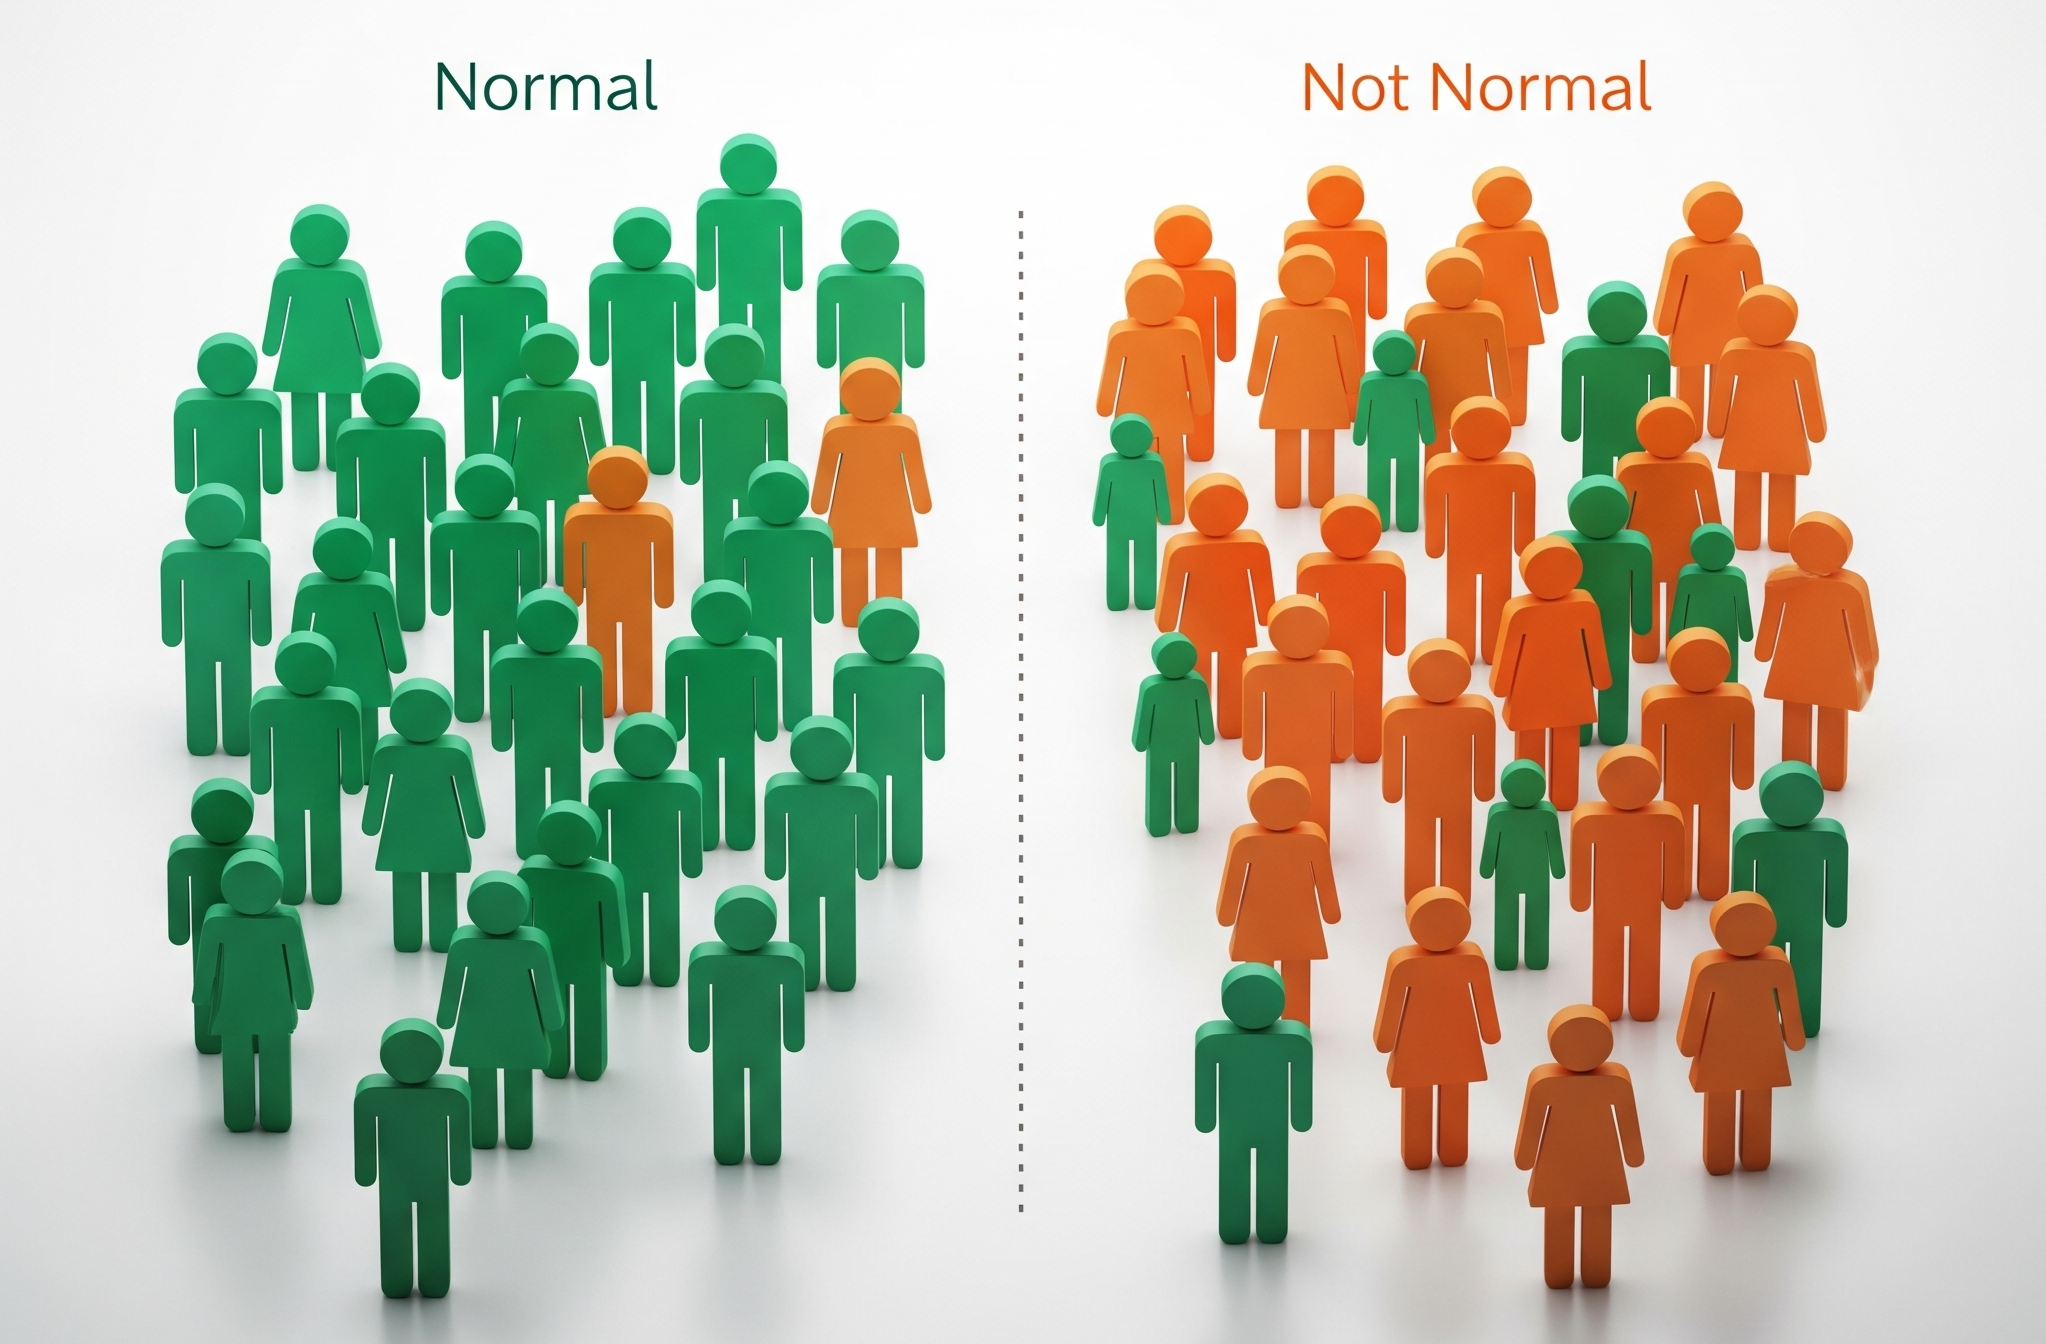
\includegraphics[width=.5\textwidth]{figures/classification.png}
	\end{center}
\end{frame}

	
% ===================================================================
\section{Case Studies and Code-Driven Examples}
% ===================================================================
	
\begin{frame}
	\frametitle{Diabetic Retinopathy Screening Agent}
	\begin{itemize}
		\item \textbf{Performance}: High accuracy and recall for detecting signs of retinopathy. Minimize false negatives.
		\item \textbf{Environment}: Primary care clinic.
		\item \textbf{Actuators}: A classification output: ["No DR", "Mild DR", "Severe DR"]. This output flags patients for a specialist.
		\item \textbf{Sensors}: A fundus camera capturing retinal images. Or an ERG machine measuring retinal function.
	\end{itemize}
	\begin{alertblock}{Agent Function}
		The function is a machine learning model (e.g., a Convolutional Neural Network) that takes a retinal image as input and outputs a diagnostic class.
	\end{alertblock}
\end{frame}
	

\begin{frame}[fragile]
	\frametitle{EEG Analysis with MNE-Python}
	\textbf{Goal}: Remove eye-blink artifacts from raw EEG data using Independent Component Analysis (ICA).
	\begin{itemize}
		\item \textbf{Sensors}: EEG electrodes.
		\item \textbf{Action}: Produce a clean EEG signal for further analysis (e.g., ERP or spectral analysis).
		\item \textbf{Tool}: MNE-Python (\textit{Magnetic and Electric Neuroimaging}) is a powerful library for EEG/MEG analysis.
	\end{itemize}
	\begin{alertblock}{The Code}
		The following script loads sample data, applies ICA, identifies and removes EOG (electrooculogram) components, and prepares the data for visualization.
	\end{alertblock}
\end{frame}

\begin{frame}
	\frametitle{EEG Analysis: Expected Output}
	\begin{figure}
		\centering
		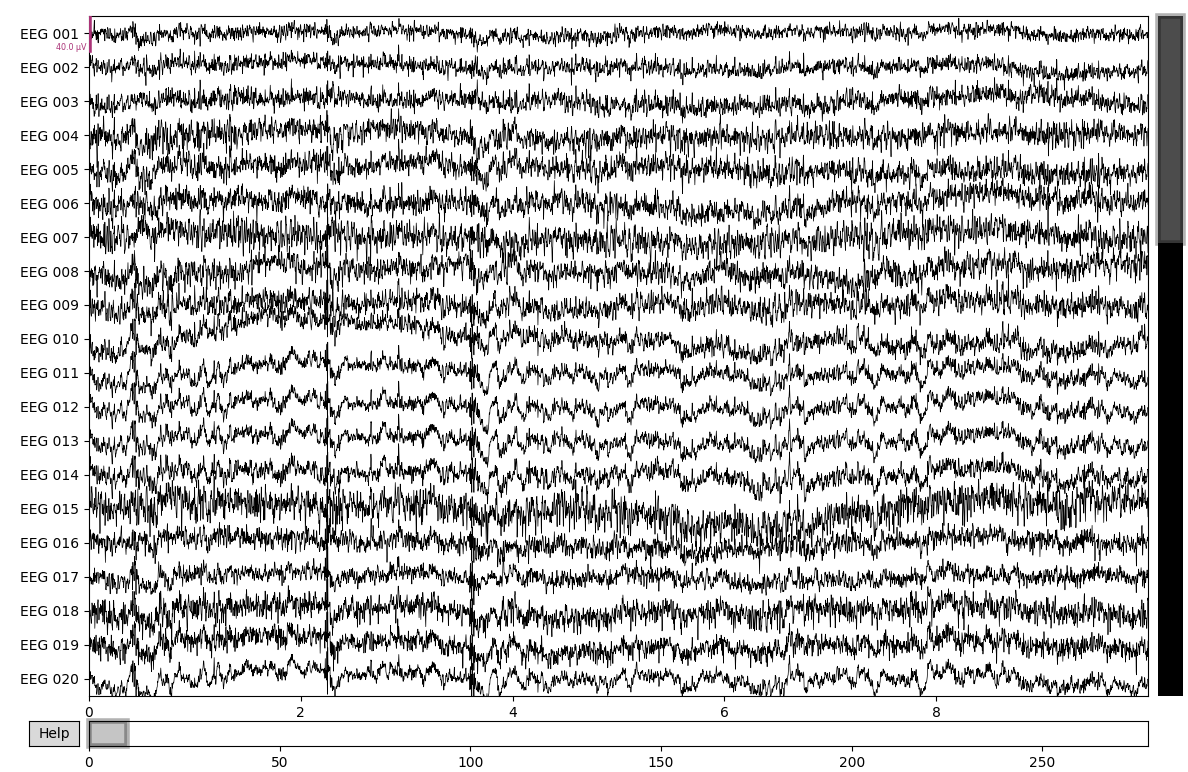
\includegraphics[width=\textheight]{figures/mne_eeg.png}
		\caption{Cleaned EEG data ready for scientific analysis.}
	\end{figure}
\end{frame}
	
	
\begin{frame}[fragile]
	\frametitle{fMRI Analysis with Nilearn}
	\textbf{Goal}: Decode what a person is seeing (face vs. house) based on brain activity in the ventral temporal (VT) cortex.
	\begin{itemize}
		\item \textbf{Performance}: Classification accuracy.
		\item \textbf{Environment}: Haxby dataset of fMRI responses to visual categories.
		\item \textbf{Actuator}: Predict the visual stimulus category.
		\item \textbf{Sensor}: fMRI scanner.
		\item \textbf{Tool}: Nilearn and Scikit-learn for machine learning on neuroimaging data.
	\end{itemize}
\end{frame}


\begin{frame}
	\frametitle{fMRI Analysis: Expected Output}
	\begin{figure}
		\centering
		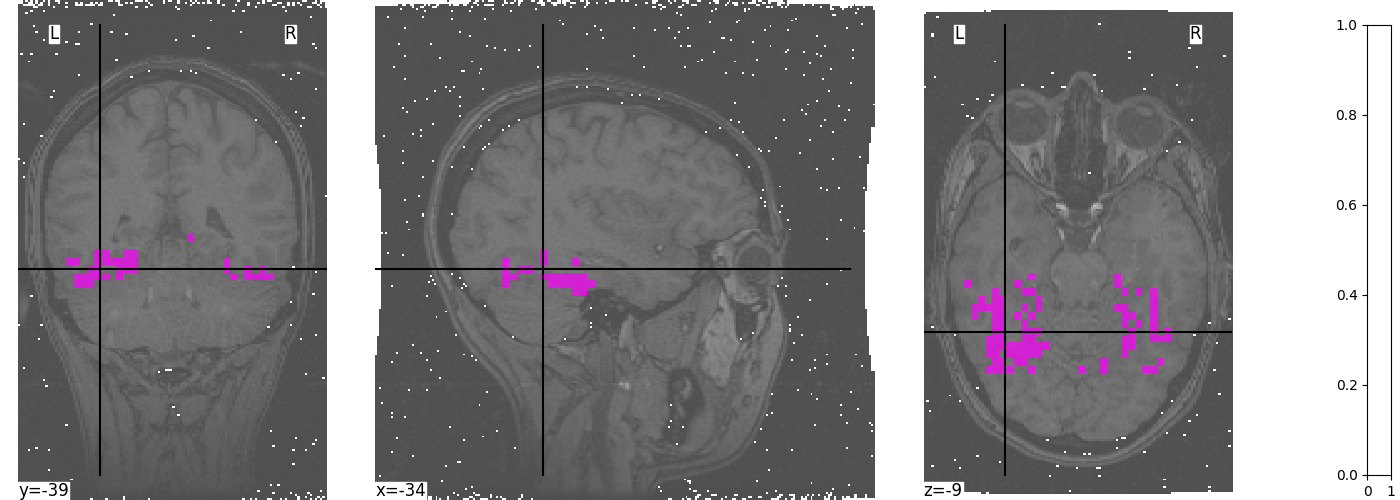
\includegraphics[width=\textwidth]{figures/fmri_vt_mask.png}
		\caption{Brain voxel data from 4D fMRI images. Uses ventral temporal cortex mask to focus on visual processing}
	\end{figure}
\end{frame}




\begin{frame}
	\frametitle{fMRI Analysis: Expected Output}
	\begin{columns}
		\begin{column}{0.6\textwidth}
			\footnotesize
		\begin{tabular}{lccc}
			\hline
			\textbf{Class} & \textbf{Precision} & \textbf{Recall} & \textbf{F1-score} \\
			\hline
			bottle        & 0.69 & 0.79 & 0.73 \\
			cat           & 0.80 & 0.91 & 0.85 \\
			chair         & 0.87 & 0.95 & 0.91 \\
			face          & 0.94 & 0.71 & 0.81 \\
			house         & 1.00 & 0.95 & 0.97 \\
			rest          & 0.95 & 0.96 & 0.96 \\
			scissors      & 0.87 & 0.91 & 0.89 \\
			scrambledpix  & 0.96 & 0.96 & 0.96 \\
			shoe          & 0.81 & 0.72 & 0.76 \\
			\hline
			\textbf{accuracy}     &      &      & 0.91 \\
			\textbf{macro avg}    & 0.88 & 0.87 & 0.87 \\
			\textbf{wgtd avg}     & 0.91 & 0.91 & 0.91 \\
			\hline
		\end{tabular}
		\end{column}
		\begin{column}{0.4\textwidth}
			\begin{figure}
				\centering
				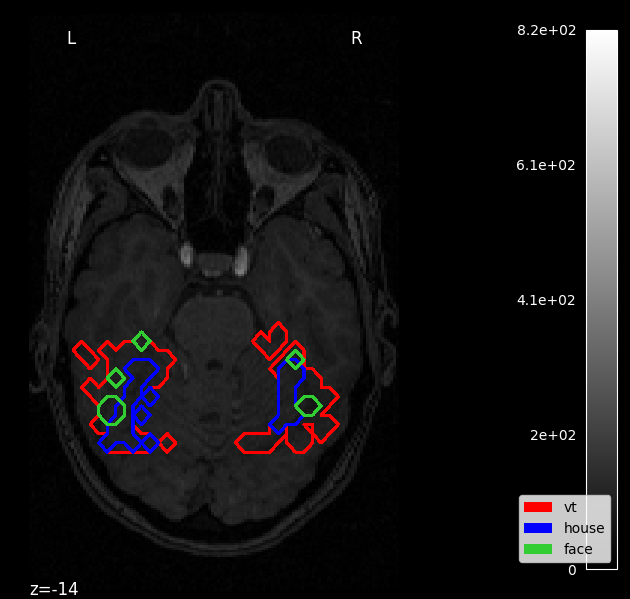
\includegraphics[width=.9\textwidth]{figures/fmri_vt_classification.png}
			\end{figure}
		\end{column}
	\end{columns}
\end{frame}
	
	
\begin{frame}[fragile]
	\frametitle{ERG Analysis with Python}
	\textbf{Goal}: Classify subjects as "Healthy" or "Not normal" (Glaucoma) based on Pattern Electroretinogram (PERG) signals.
	\begin{itemize}
		\item \textbf{Performance}: Classification accuracy, confusion matrix.
		\item \textbf{Environment}: PERG-IOBA dataset.
		\item \textbf{Actuator}: Diagnostic label ("Healthy" / "Not normal").
		\item \textbf{Sensor}: PERG recording system.
		\item \textbf{Tools}: Pandas, Scikit-learn, Imblearn.
	\end{itemize}
\end{frame}
	
\begin{frame}
	\frametitle{ERG Analysis: Dataset}
\begin{figure}
	\centering
	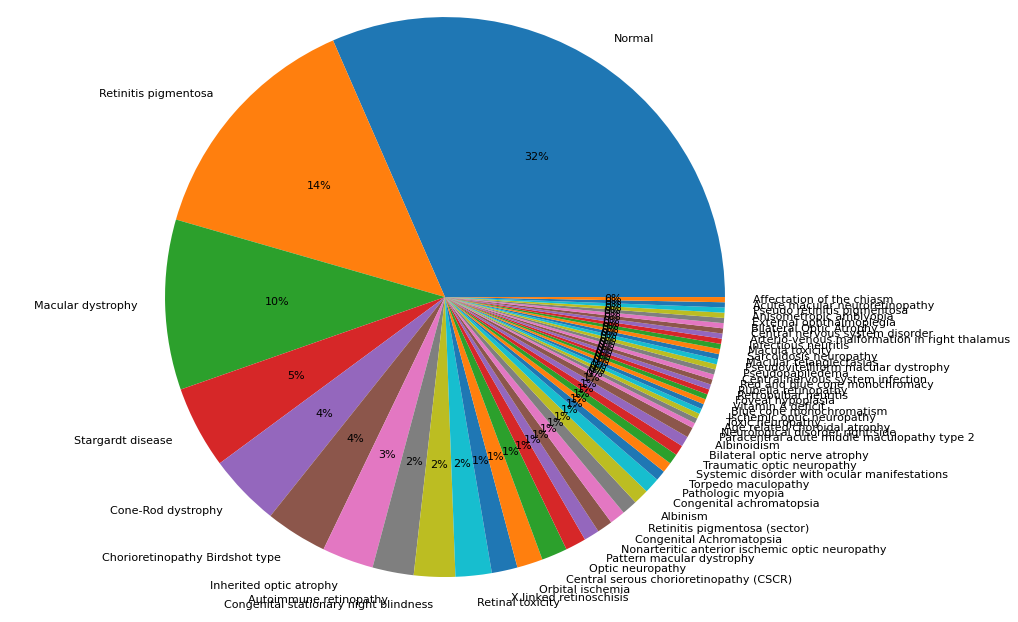
\includegraphics[width=.9\textwidth]{figures/perg_group_distribution_pie.png}
	\caption{Group distribution dataset}
	\label{fig:perggroupdistributionpie}
\end{figure}
\end{frame}
	

\begin{frame}
	\frametitle{ERG Analysis: Feature Extraction}
	\begin{tabular}{p{0.5\textwidth}p{0.5\textwidth}}
			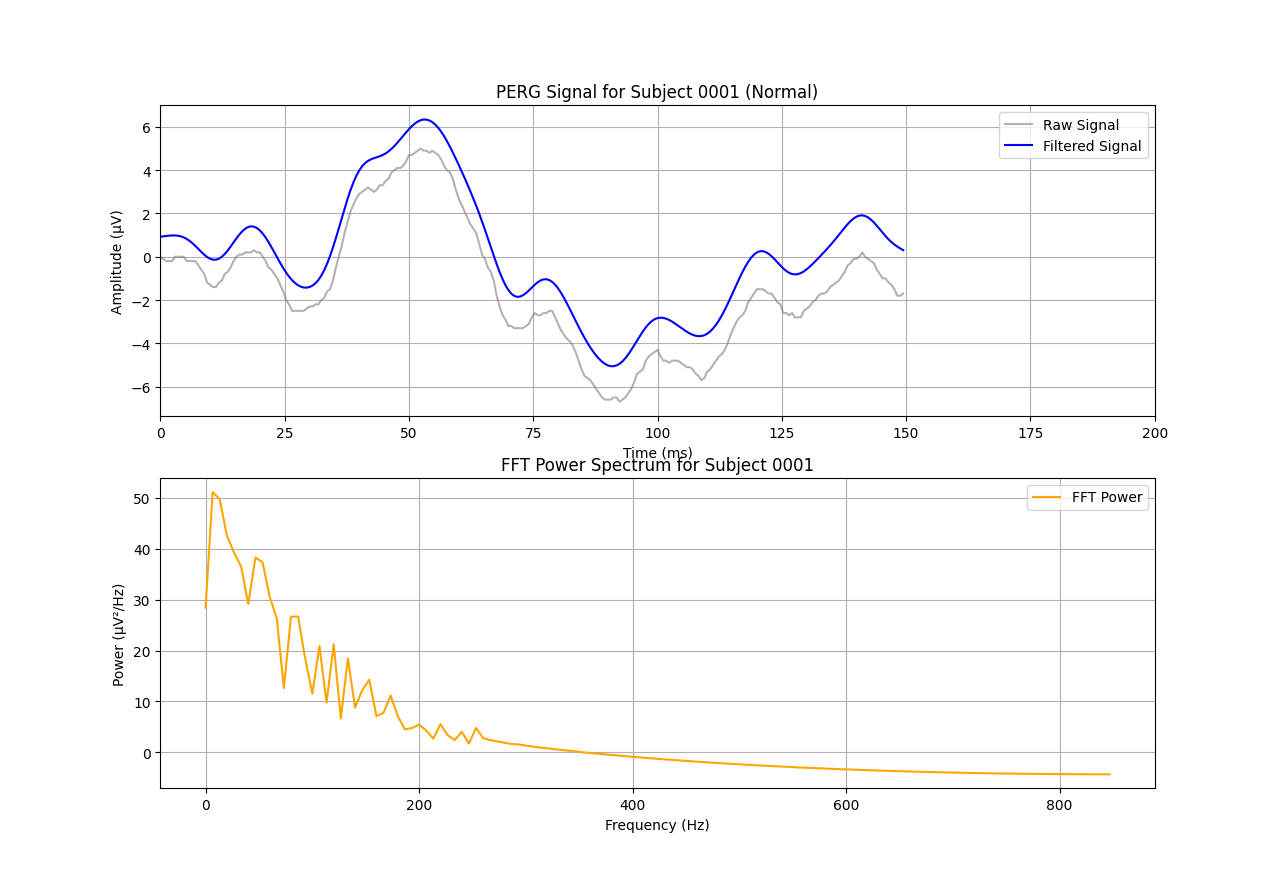
\includegraphics[width=.45\textwidth]{figures/perg_sub0001.png} & 
			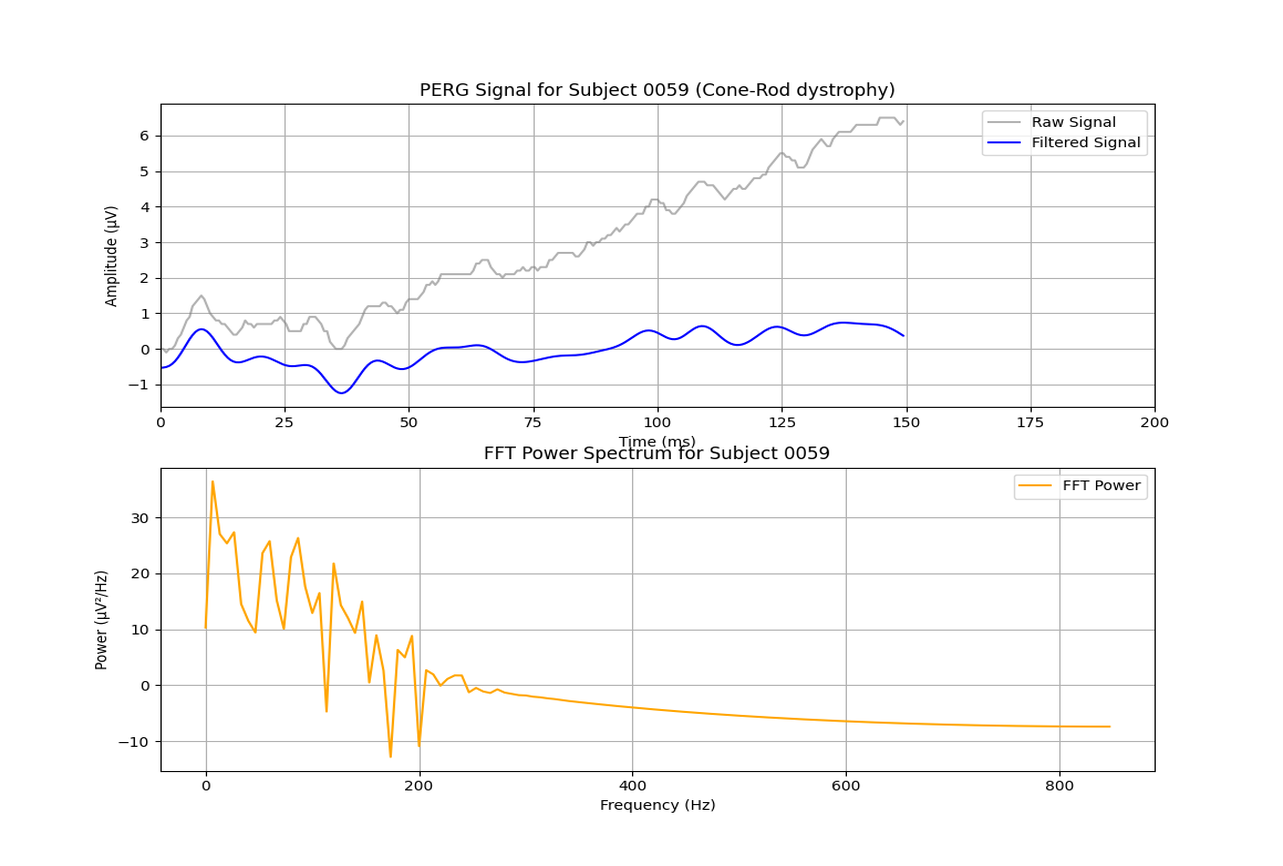
\includegraphics[width=.45\textwidth]{figures/perg_sub0059.png}
			\\ 
			{\small Healthy subject} & 
			{\small Impaired subject}
			\\
			{\small (a) Sample PERG Waveform.} & 
			{\small (a) Sample PERG Waveform.}
			\\
			{\small (b) Power Spectrum in dB.} & 
			{\small (b) Power Spectrum in dB.}
	\end{tabular}
\end{frame}

\begin{frame}
	\frametitle{ERG Analysis: Expected Output}
	\begin{columns}
		\begin{column}{0.5\textwidth}
			\begin{table}[h!]
				\centering
				\begin{tabular}{lcccc}
					\hline
					\textbf{Class} & \textbf{Precision} & \textbf{Recall} & \textbf{F1-score} & \textbf{Support} \\
					\hline
					Healthy      & 0.74 & 0.81 & 0.77 & 69 \\
					Not normal   & 0.79 & 0.71 & 0.75 & 69 \\
					\hline
					\textbf{accuracy}     &      &      & 0.76 & 138 \\
					\textbf{macro avg}    & 0.76 & 0.76 & 0.76 & 138 \\
					\textbf{weighted avg} & 0.76 & 0.76 & 0.76 & 138 \\
					\hline
				\end{tabular}
				\caption{Classification report for Healthy vs Not normal}
				\label{tab:classification_report_healthy}
			\end{table}
		\end{column}
		\begin{column}{0.5\textwidth}
			\begin{figure}
				\centering
				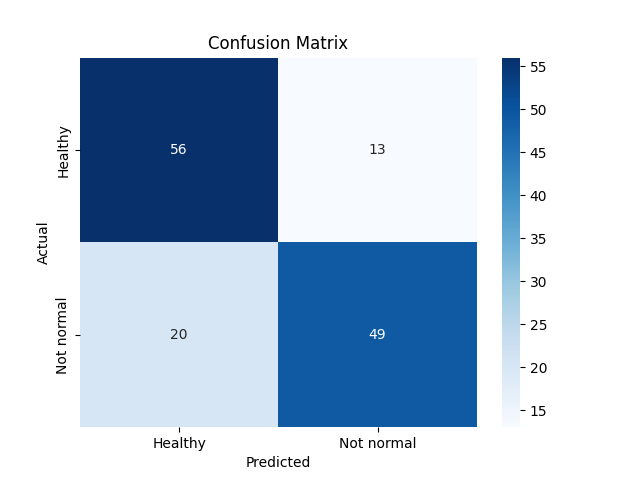
\includegraphics[width=\textwidth]{figures/perg_confusion_matrix.png}
				\caption{Confusion Matrix}
				\label{fig:pergconfusionmatrix}
			\end{figure}
		\end{column}
	\end{columns}
\end{frame}


% ===================================================================
\section{Links to Real Datasets}
% ===================================================================

\begin{frame}
	\frametitle{Explore Real-World Data}
	You can apply these methods to publicly available datasets.
	\begin{itemize}
		\item \textbf{EEG}:
		\begin{itemize}
			\item \href{https://openneuro.org/datasets/ds003190}{OpenNeuro: ds003190} - P300 paradigm
		\end{itemize}
		\item \textbf{fMRI}:
		\begin{itemize}
			\item \href{https://openneuro.org/datasets/ds004496}{OpenNeuro: ds004496} - Natural images and words
		\end{itemize}
		\item \textbf{Eye-Tracking}:
		\begin{itemize}
			\item \href{https://www.kaggle.com/datasets/imtkaggleteam/eye-tracking-autism}{Kaggle: Eye Tracking Autism}
		\end{itemize}
		\item \textbf{ERG}:
		\begin{itemize}
			\item \href{https://physionet.org/content/perg-ioba-dataset/1.0.0/}{PhysioNet: PERG Database from IOBA}
		\end{itemize}
	\end{itemize}
\end{frame}


% ===================================================================
\section{Conclusion}
% ===================================================================

\begin{frame}
	\frametitle{Thank You}
	\begin{center}
		\Huge Thank You!
		\vspace{1cm}
		
		\Large Questions?
		\vspace{1cm}
		
		\small Contact: \url{lapan.hugodepaula@gmail.com} \\
		\small Website: \url{lapan.com.br}
		\vspace{1cm}
		
		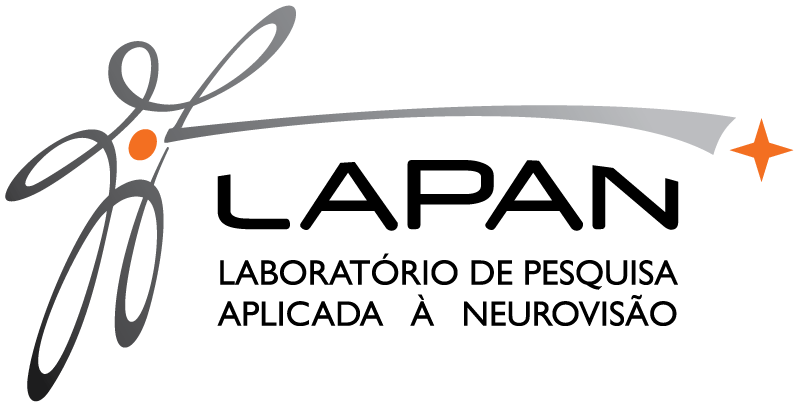
\includegraphics[height=2cm]{lapan.png}
	\end{center}
\end{frame}
	
	
\end{document}